\documentclass{article}
\usepackage[utf8]{inputenc}
\usepackage{amsmath}
\usepackage{graphicx}
\usepackage{titling}

\title{\textbf{\Huge NLP Assignment 2: Answers}}
\author{Name: Alireza Dastmalchi Saei}
\date{Stu No.: 993613026}

\pretitle{%
  \begin{center}
  \includegraphics[width = 150px]{Images/university-of-isfahan-logo.png}\\[\bigskipamount]
  \vspace{3cm}
}
\posttitle{\end{center}}

\begin{document}
\maketitle

\pagebreak

\section*{POS Tagging}
\subsection{Probability Table}
First, the count matrix must be calculated to:
\begin{table}[htbp]
    \centering
    \caption{Count Table}
    \renewcommand{\arraystretch}{1.5}
    \begin{tabular}{|c|c|c|c|}
        \hline
        \textbf{Words Count} & \textbf{Noun} & \textbf{Modal} & \textbf{Verb} \\
        \hline
        \text{Mark} & 1 & 0 & 2 \\
        \text{Can} & 0 & 3 & 0 \\
        \text{Watch} & 2 & 0 & 2 \\
        \text{Tom} & 2 & 0 & 0 \\
        \text{Will} & 1 & 1 & 0 \\
        \hline
    \end{tabular}
    \label{tab:count-table}
\end{table}

Now that we have the count vector, the probability table of each word being Noun, Model, or Verb will be as follows:
\begin{table}[htbp]
    \centering
    \caption{Probability Table}
    \renewcommand{\arraystretch}{1.5}
    \begin{tabular}{|c|c|c|c|}
        \hline
        \textbf{Words Probs} & \textbf{Noun} & \textbf{Modal} & \textbf{Verb} \\
        \hline
        \text{Mark} & $\frac{1}{6}$ & 0 & $\frac{1}{2}$ \\
        \text{Can} & 0 & $\frac{3}{4}$ & 0 \\
        \text{Watch} & $\frac{2}{6}$ & 0 & $\frac{1}{2}$ \\
        \text{Tom} & $\frac{2}{6}$ & 0 & 0 \\
        \text{Will} & $\frac{1}{6}$ & $\frac{1}{4}$ & 0 \\
        \hline
    \end{tabular}
    \label{tab:probability-table}
\end{table}

\pagebreak

\subsection{Sentences with \textless S\textgreater and \textless E\textgreater}
Sentences are with Start and End Sentence Tags are:
\begin{itemize}
  \item \textless S\textgreater Mark can watch \textless E\textgreater (S N M V E)
  \item \textless S\textgreater Will can mark watch \textless E\textgreater (S N M V N E)
  \item \textless S\textgreater Can Tom watch? \textless E\textgreater (S M N V E)
  \item \textless S\textgreater Tom will mark watch \textless E\textgreater (S N M V N E)
\end{itemize}

Now with these new sentences the below count table can be created:
\begin{table}[htbp]
    \centering
    \caption{Occurrence Table}
    \renewcommand{\arraystretch}{1.5}
    \begin{tabular}{|c|c|c|c|c|}
        \hline
        \textbf{} & \textbf{Noun} & \textbf{Modal} & \textbf{Verb} & \textbf{\textless E\textgreater} \\
        \hline
        \textbf{\textless S\textgreater} & 3 & 1 & 0 & 0 \\
        \textbf{Noun} & 0 & 3 & 1 & 2 \\
        \textbf{Modal} & 1 & 0 & 3 & 0 \\
        \textbf{Verb} & 2 & 0 & 0 & 2 \\
        \hline
    \end{tabular}
    \label{tab:occ-table}
\end{table}

Now by dividing each number by sum of row numbers, we will get probabilities happening specific POS sequences:
\begin{table}[htbp]
    \centering
    \caption{Prob. Occurrence Table}
    \renewcommand{\arraystretch}{1.5}
    \begin{tabular}{|c|c|c|c|c|}
        \hline
        \textbf{} & \textbf{Noun} & \textbf{Modal} & \textbf{Verb} & \textbf{\textless E\textgreater} \\
        \hline
        \textbf{\textless S\textgreater} & $\frac{3}{4}$ & $\frac{1}{4}$ & 0 & 0 \\
        \textbf{Noun} & 0 & $\frac{1}{2}$ & $\frac{1}{6}$ & $\frac{1}{3}$ \\
        \textbf{Modal} & $\frac{1}{4}$ & 0 & $\frac{3}{4}$ & 0 \\
        \textbf{Verb} & $\frac{1}{2}$ & 0 & 0 & $\frac{1}{2}$ \\
        \hline
    \end{tabular}
    \label{tab:prob-occ-table}
\end{table}

\pagebreak

\subsection{Applying POS Tagging}
The sentence is "Can Tom mark watch" and the POS tagging must result:

\textbf{\textless S\textgreater Modal Noun Verb Noun \textless E\textgreater}

\begin{figure}[htbp]
    \centering
    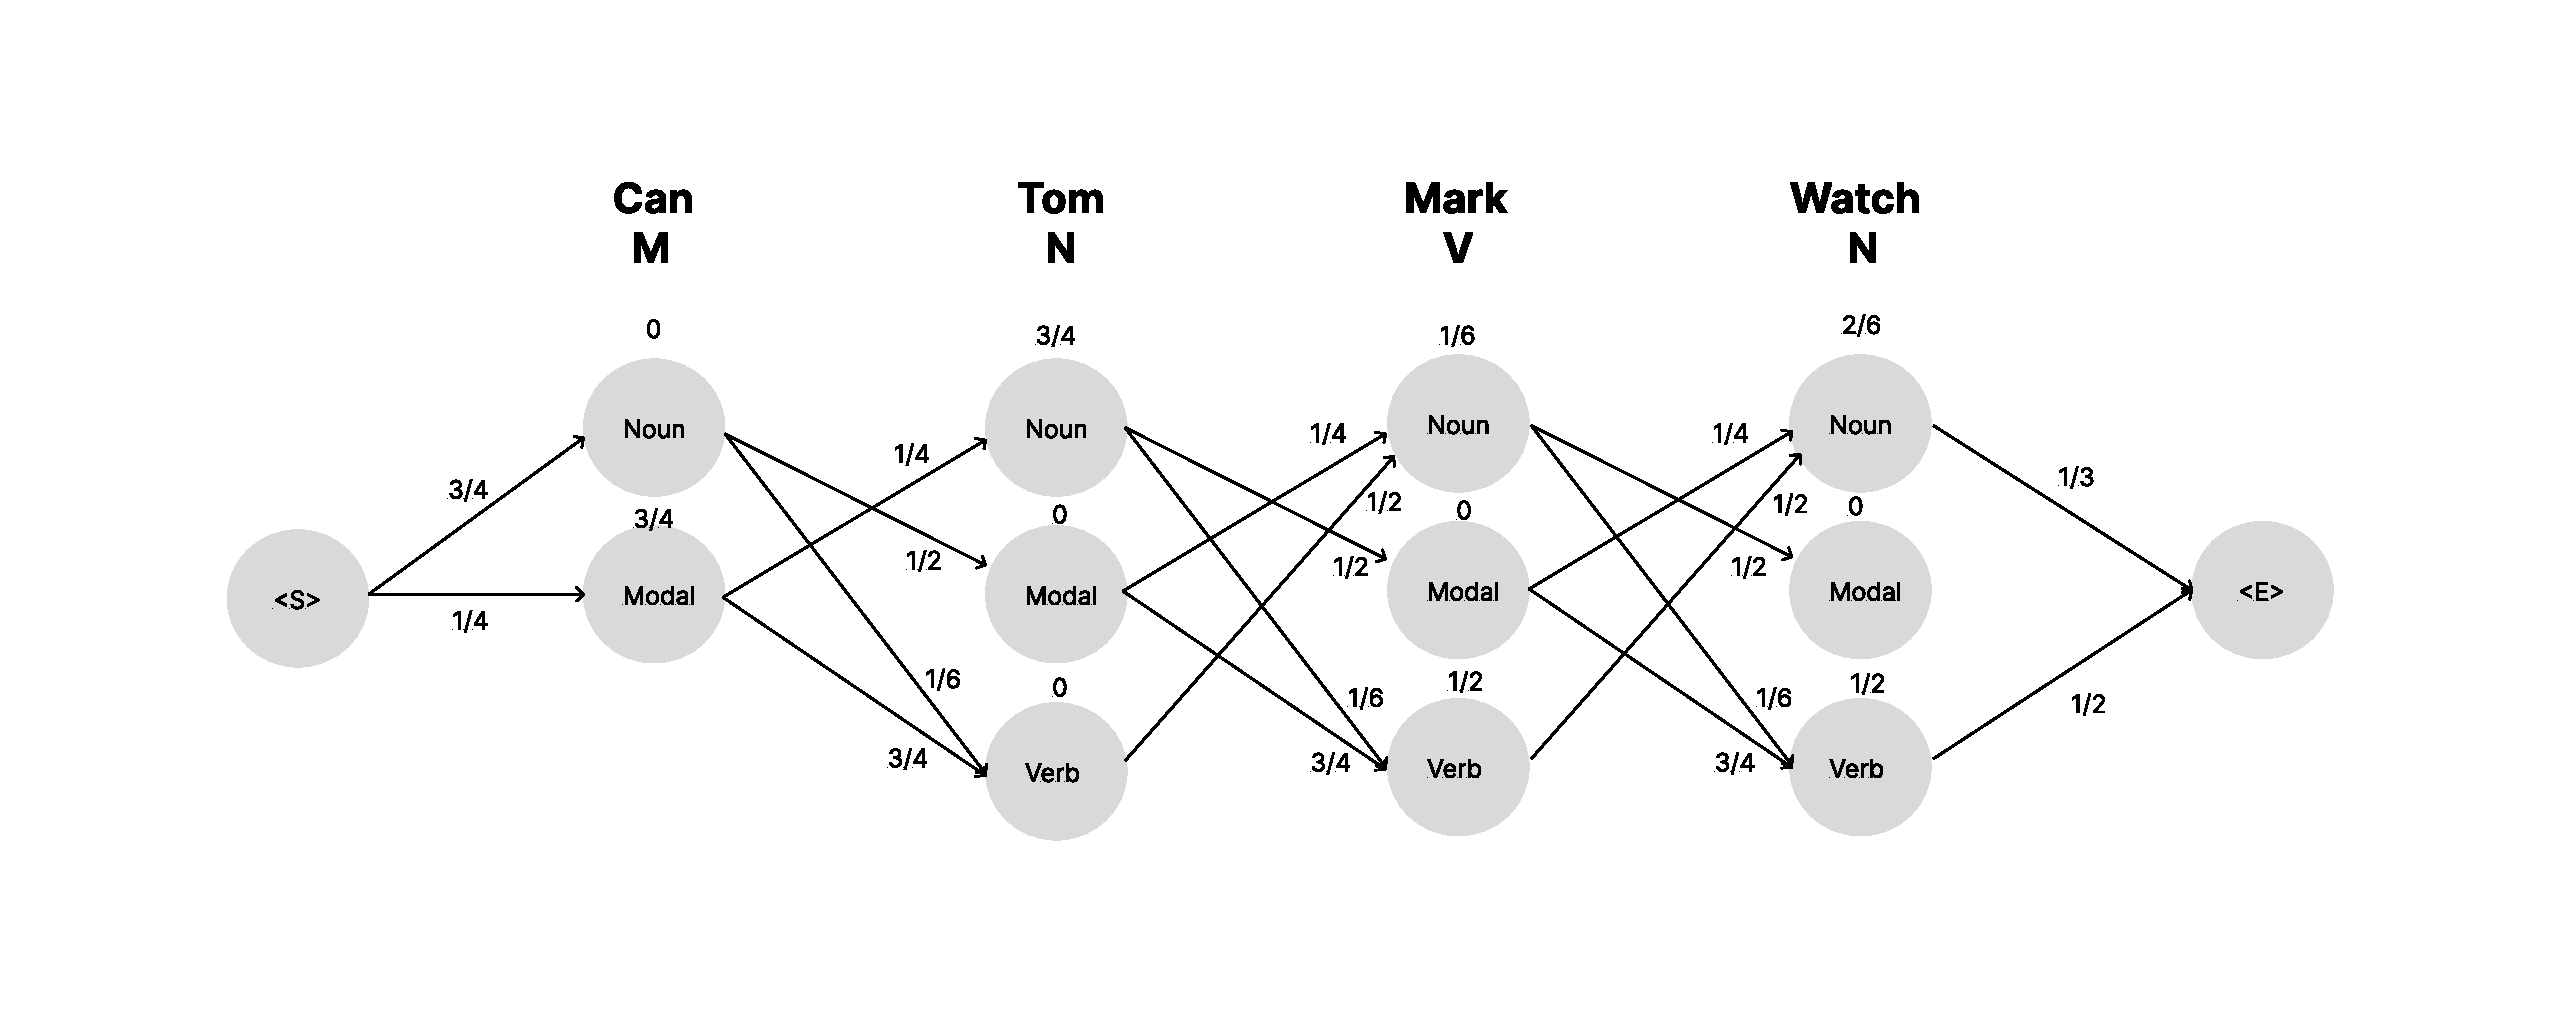
\includegraphics[width=1\textwidth]{Images/HMM.pdf}
    \caption{Hidden Markov Model for the given Sentence}
    \label{fig:HMM}
\end{figure}


\begin{figure}[htbp]
    \centering
    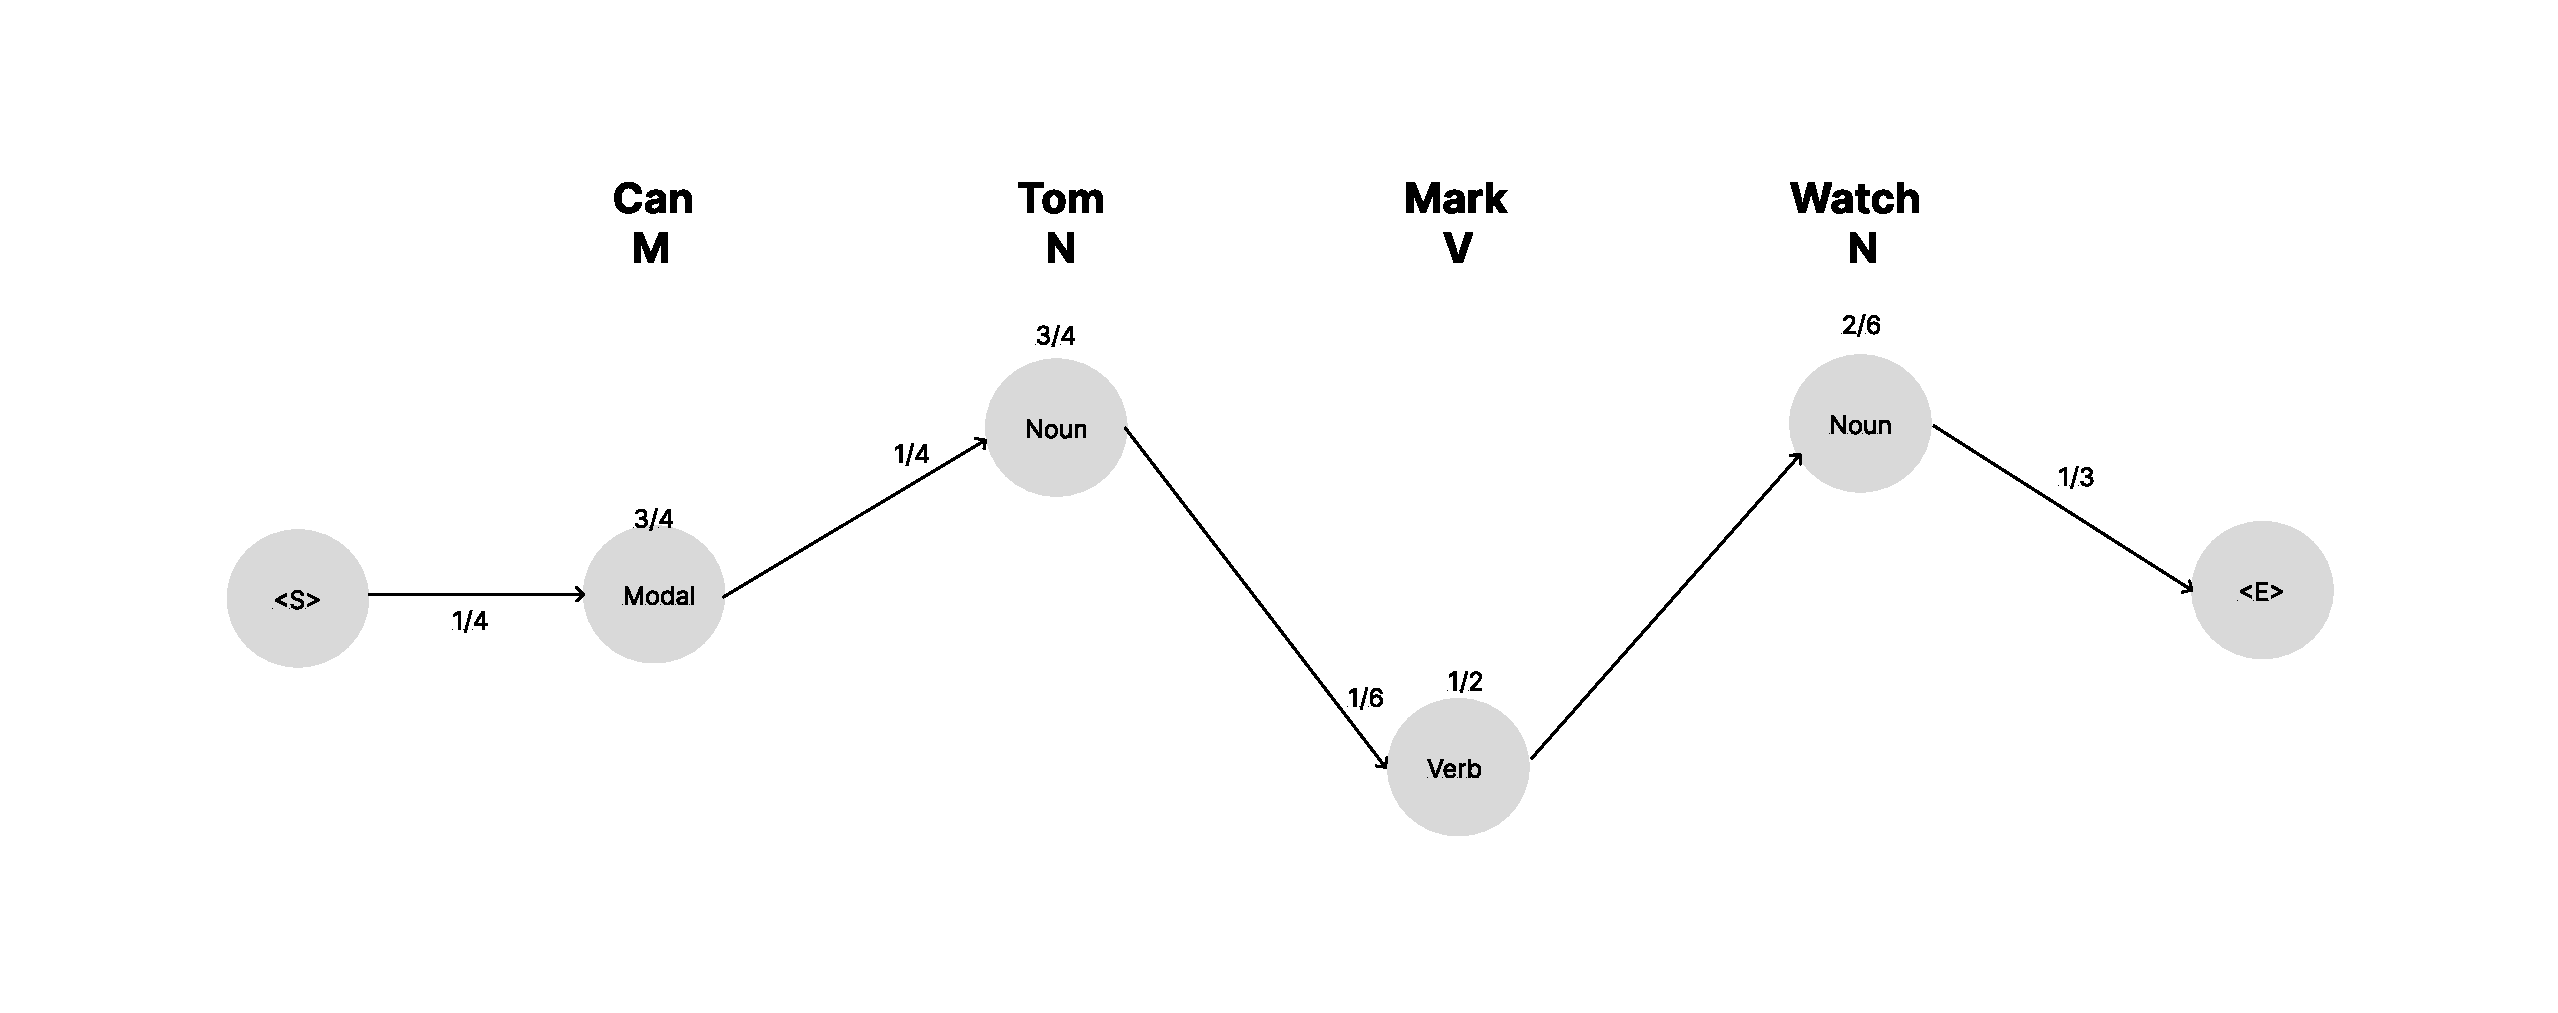
\includegraphics[width=1\textwidth]{Images/HMM_Simplified.pdf}
    \caption{Simplified Hidden Markov Model}
    \label{fig:HMM}
\end{figure}

\bigskip
\bigskip
\bigskip


\begin{align*}
\text{P(Sentence)} &= \frac{1}{4} \times \frac{3}{4} \times \frac{1}{4} \times \frac{3}{4} \times \frac{1}{6} \times \frac{1}{2} \times \frac{1}{2} \times \frac{2}{6} \times \frac{1}{3} \\
&= 0.0001627604
\end{align*}

\end{document}
